\documentclass[aspectratio=169,11pt]{beamer}

\usepackage[utf8]{inputenc}
\usepackage[T1]{fontenc}
\usepackage{lmodern}
\usepackage{xcolor}
\usepackage{tikz}
\usepackage{listings}
\usepackage{booktabs}
\usepackage{array}
\usepackage{pifont}
\usepackage{fontawesome5}
\usetikzlibrary{shapes.geometric, arrows.meta, positioning, shadows, fit, backgrounds, calc}

%======================================================================
%  GeoSI Brand Palette
%======================================================================
\definecolor{geosinavy}{HTML}{0B2A4A}
\definecolor{geositeal}{HTML}{108A92}
\definecolor{geosimuted}{HTML}{555F6D}
\definecolor{geosisand}{HTML}{F4F1EA}
\definecolor{geosiamber}{HTML}{E2A93B}
\definecolor{geosigreen}{HTML}{2F8F6B}
\definecolor{geosired}{HTML}{C0564A}
\definecolor{geosilight}{HTML}{E8EEF2}

%======================================================================
%  Beamer Theme
%======================================================================
\usetheme{default}
\usecolortheme{default}
\setbeamercolor{structure}{fg=geosinavy}
\setbeamercolor{frametitle}{fg=white,bg=geosinavy}
\setbeamercolor{title}{fg=geosinavy}
\setbeamercolor{subtitle}{fg=geositeal}
\setbeamercolor{author}{fg=geosimuted}
\setbeamercolor{institute}{fg=geosimuted}
\setbeamercolor{date}{fg=geosimuted}
\setbeamercolor{normal text}{fg=geosinavy}
\setbeamercolor{itemize item}{fg=geositeal}
\setbeamercolor{itemize subitem}{fg=geosiamber}
\setbeamercolor{block title}{fg=white,bg=geositeal}
\setbeamercolor{block body}{bg=geosisand,fg=geosinavy}
\setbeamerfont{frametitle}{series=\bfseries,size=\large}
\setbeamerfont{title}{series=\bfseries,size=\huge}
\setbeamertemplate{navigation symbols}{}
\setbeamertemplate{itemize item}{\small\raise0.5pt\hbox{\textbullet}}
\setbeamertemplate{itemize subitem}{\small\raise0.5pt\hbox{\textendash}}

% Frame title bar
\setbeamertemplate{frametitle}{%
  \nointerlineskip
  \begin{beamercolorbox}[wd=\paperwidth,ht=3.2ex,dp=1.2ex,leftskip=0.9em,rightskip=0.9em]{frametitle}
    \strut\insertframetitle\strut\hfill{\small\color{geosisand}\insertframenumber\,/\,20}
  \end{beamercolorbox}%
  \vskip4pt
}

% Footer
\setbeamertemplate{footline}{%
  \leavevmode
  \hbox to \paperwidth{%
    \hspace{0.9em}\color{geosimuted}\scriptsize GeoSI \textbullet\ Geospatial Superintelligence \textbullet\ v2.0
    \hfill
    \color{geosimuted}\scriptsize Aaron R \textbullet\ Digital University Kerala \hspace{0.9em}%
  }\vskip4pt
}

%======================================================================
%  Listings
%======================================================================
\lstset{
  basicstyle=\ttfamily\footnotesize\color{geosinavy},
  backgroundcolor=\color{geosisand},
  frame=single,
  rulecolor=\color{geositeal},
  keywordstyle=\color{geositeal}\bfseries,
  commentstyle=\color{geosimuted}\itshape,
  stringstyle=\color{geosigreen},
  breaklines=true,
  columns=fullflexible,
  keepspaces=true,
  xleftmargin=6pt,
  xrightmargin=6pt,
  framesep=6pt,
  aboveskip=4pt,
  belowskip=4pt,
}

\lstdefinestyle{chat}{
  basicstyle=\ttfamily\footnotesize\color{geosinavy},
  backgroundcolor=\color{geosilight},
  frame=leftline,
  rulecolor=\color{geosiamber},
  breaklines=true,
}

%======================================================================
%  Helper Commands
%======================================================================
\newcommand{\chip}[2]{%
  \tikz[baseline=(a.base)]\node[draw=#1,fill=#1!10,text=#1,rounded corners=3pt,inner sep=3pt,font=\scriptsize\bfseries] (a) {#2};%
}
\newcommand{\kw}[1]{{\color{geositeal}\bfseries #1}}

%======================================================================
%  Metadata
%======================================================================
\title{GeoSI}
\subtitle{The Beginning of Geospatial Superintelligence\\[0.15em]\normalsize\mdseries A Conversational Multi-Tool Engine for Professional GIS}
\author{Aaron R}
\institute{Digital University Kerala (DUK)\\ \texttt{aaronr.ds25@duk.ac.in}}
\date{May 2026 \ \textbullet\ \ Version 2.0}

\begin{document}

%======================================================================
%  SLIDE 1 --- TITLE
%======================================================================
{
\setbeamertemplate{footline}{}
\begin{frame}[plain]
  \begin{tikzpicture}[remember picture, overlay]
    \fill[geosinavy] (current page.north west) rectangle (current page.south east);
    \fill[geositeal, opacity=0.18]
      ([xshift=-2cm,yshift=-1.5cm]current page.north east)
      circle (6cm);
    \fill[geosiamber, opacity=0.15]
      ([xshift=1.5cm,yshift=2cm]current page.south west)
      circle (4.5cm);

    \node[anchor=north west, xshift=0.9cm, yshift=-1.3cm] at (current page.north west)
      {\color{geosiamber}\scriptsize\bfseries DIGITAL UNIVERSITY KERALA \ \textbullet\ \ 2026};

    \node[anchor=west, xshift=1cm, yshift=1.2cm] at (current page.west)
      {\begin{minipage}{0.85\paperwidth}
        {\color{white}\fontsize{64pt}{70pt}\selectfont\bfseries GeoSI}\\[0.2em]
        {\color{geosiamber}\Large\bfseries The Beginning of Geospatial Superintelligence}\\[0.3em]
        {\color{geosilight}\normalsize A Conversational Multi-Tool Engine for Professional GIS}
      \end{minipage}};

    \node[anchor=south west, xshift=1cm, yshift=1cm] at (current page.south west)
      {\begin{minipage}{0.8\paperwidth}
        {\color{white}\normalsize\bfseries Aaron R}\\
        {\color{geosilight}\small Digital University Kerala}\\
        {\color{geosilight}\small aaronr.ds25@duk.ac.in}
      \end{minipage}};

    \node[anchor=south east, xshift=-1cm, yshift=1cm] at (current page.south east)
      {\color{geosilight}\small May 2026 \ \textbullet\ \ v2.0};
  \end{tikzpicture}
\end{frame}
}

%======================================================================
%  SLIDE 2 --- THE PROBLEM
%======================================================================
\begin{frame}{The Problem: GIS Is Powerful But Locked Behind Complexity}
  \begin{columns}[T,onlytextwidth]
    \begin{column}{0.55\textwidth}
      \small
      \begin{block}{The Expert Gap}
        Professional GIS is indispensable for \kw{urban planning}, \kw{disaster response}, \kw{agriculture}, \kw{conservation}, and \kw{public policy} --- yet the cognitive overhead remains painfully high.
      \end{block}
      \vspace{0.3em}
      \textbf{Today, answering a spatial question requires fluency in:}
      \begin{itemize}
        \item Hundreds of algorithms and their parameters
        \item Coordinate reference systems (CRS) and projections
        \item Vendor-specific menus, scripts, and query languages
        \item Toolchain ordering and intermediate data handling
      \end{itemize}
      \vspace{0.2em}
      \textbf{The result:} domain experts who understand \emph{the question} depend on GIS analysts to produce \emph{the answer}.
    \end{column}
    \begin{column}{0.45\textwidth}
      \centering
      \begin{tikzpicture}[node distance=0.4cm]
        \node[draw=geosinavy, fill=geosilight, rounded corners, text width=3.6cm, align=center, font=\small\bfseries, minimum height=0.9cm] (q) {Spatial Question\\\small\mdseries ``sites within 500m of hospitals''};
        \node[draw=geosired, fill=geosired!10, rounded corners, below=of q, text width=3.6cm, align=center, font=\small] (wall) {\color{geosired}\faExclamationTriangle\ \textbf{Wall of Complexity}\\\scriptsize menus \textbullet\ scripts \textbullet\ CRS \textbullet\ SQL};
        \node[draw=geosimuted, fill=geosisand, rounded corners, below=of wall, text width=3.6cm, align=center, font=\small] (ana) {GIS Analyst\\\scriptsize (bottleneck)};
        \node[draw=geositeal, fill=geositeal!10, rounded corners, below=of ana, text width=3.6cm, align=center, font=\small\bfseries] (ans) {Answer};
        \draw[-{Stealth},thick,geosinavy] (q) -- (wall);
        \draw[-{Stealth},thick,geosimuted] (wall) -- (ana);
        \draw[-{Stealth},thick,geositeal] (ana) -- (ans);
      \end{tikzpicture}

      \vspace{0.4em}
      \scriptsize\color{geosimuted}\textit{General-purpose AI chatbots can describe GIS operations, but cannot execute them on your data.}
    \end{column}
  \end{columns}
\end{frame}

%======================================================================
%  SLIDE 3 --- WHAT IS GEOSI
%======================================================================
\begin{frame}{What Is GeoSI?}
  \begin{block}{Definition}
    \textbf{GeoSI} (Geospatial Superintelligence) is a production-ready conversational AI system that bridges natural language and professional GIS, decomposing plain-English spatial questions into multi-step workflows executed across \textbf{127 geospatial tools} on layers already loaded in the user's QGIS workspace.
  \end{block}

  \begin{columns}[T,onlytextwidth]
    \begin{column}{0.33\textwidth}
      \centering
      \tikz\node[draw=geositeal,thick,fill=geositeal!10,circle,minimum size=1.4cm,font=\Large\bfseries]{127};\\[0.3em]
      \small\textbf{Tools} across 9 GIS domains
    \end{column}
    \begin{column}{0.33\textwidth}
      \centering
      \tikz\node[draw=geosiamber,thick,fill=geosiamber!15,circle,minimum size=1.4cm,font=\Large\bfseries]{3};\\[0.3em]
      \small\textbf{Surfaces} engine, plugin, server
    \end{column}
    \begin{column}{0.33\textwidth}
      \centering
      \tikz\node[draw=geosigreen,thick,fill=geosigreen!15,circle,minimum size=1.4cm,font=\Large\bfseries]{5};\\[0.3em]
      \small\textbf{LLM providers} with graceful fallback
    \end{column}
  \end{columns}

  \vspace{0.6em}
  \textbf{Core design tenets}
  \begin{itemize}
    \item \kw{Grounded} --- never hallucinates layers; operates only on what is actually loaded
    \item \kw{Local-first} --- Ollama is the default runtime; everything else is a fallback
    \item \kw{Explainable} --- every answer shows its plan, reasoning, and per-step timing
    \item \kw{Deployable} --- zero QGIS imports in the engine; runs in QGIS, servers, or notebooks
  \end{itemize}
\end{frame}

%======================================================================
%  SLIDE 4 --- KEY CONTRIBUTIONS
%======================================================================
\begin{frame}{Key Contributions}
  \small
  \begin{columns}[T,onlytextwidth]
    \begin{column}{0.5\textwidth}
      \begin{block}{1. Three-Surface Architecture}
        Strict separation isolates QGIS dependencies to a single plugin layer; the analytical engine is framework-free and importable anywhere.
      \end{block}
      \begin{block}{2. Backend-Dispatch Pattern}
        Identical tool specifications run under QGIS Processing, a portable GeoPandas backend, or return a clear unavailability error.
      \end{block}
      \begin{block}{3. Ollama-First LLM Chain}
        1.5 s availability probing with graceful fallback through Gemini, Anthropic, OpenAI, and a deterministic keyword parser --- a fully offline default.
      \end{block}
    \end{column}
    \begin{column}{0.5\textwidth}
      \begin{block}{4. Layer-Grounding Mechanism}
        Refuses to hallucinate data: queries referencing unloaded layers receive fuzzy suggestions derived from the QGIS Layers panel.
      \end{block}
      \begin{block}{5. Unified 127-Tool Catalogue}
        Auto-discovered tools across nine GIS domains, exposed through one conversational surface.
      \end{block}
      \vspace{0.4em}
      \centering
      \chip{geosinavy}{vector} \chip{geositeal}{raster} \chip{geosigreen}{terrain} \chip{geosiamber}{network}\\[0.3em]
      \chip{geosired}{temporal} \chip{geositeal}{AI/ML} \chip{geosinavy}{cartography} \chip{geosimuted}{validation}
    \end{column}
  \end{columns}
\end{frame}

%======================================================================
%  SLIDE 5 --- THREE-SURFACE ARCHITECTURE
%======================================================================
\begin{frame}{Three-Surface Architecture}
  \centering
  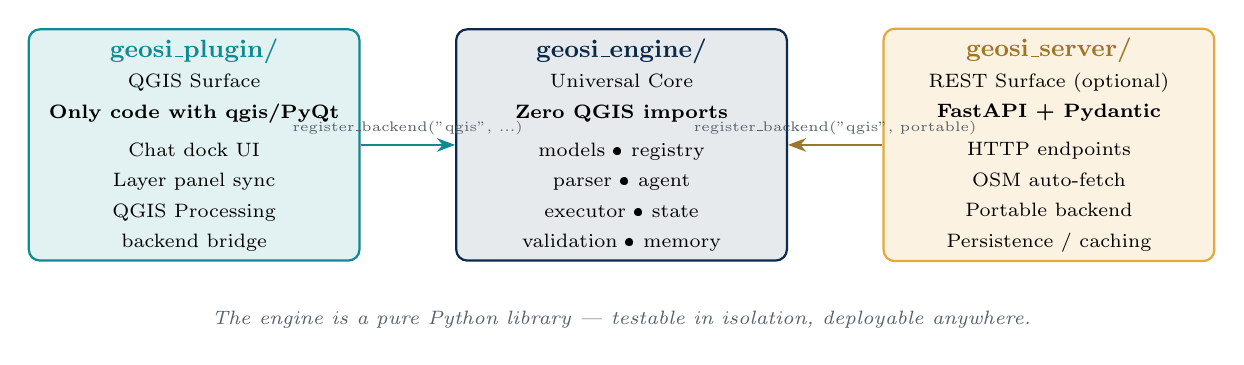
\begin{tikzpicture}[
    node distance=0.6cm and 1.2cm,
    surface/.style={draw,thick,rounded corners,minimum height=2.8cm,minimum width=4.2cm,align=center,font=\small},
    core/.style={surface,fill=geosinavy!10,draw=geosinavy},
    plugin/.style={surface,fill=geositeal!12,draw=geositeal},
    server/.style={surface,fill=geosiamber!15,draw=geosiamber},
    label/.style={font=\bfseries\small},
  ]
    \node[core] (engine) {%
      \textbf{\color{geosinavy}geosi\_engine/}\\
      \scriptsize Universal Core\\
      \scriptsize \textbf{Zero QGIS imports}\\[0.3em]
      \scriptsize models \textbullet\ registry\\
      \scriptsize parser \textbullet\ agent\\
      \scriptsize executor \textbullet\ state\\
      \scriptsize validation \textbullet\ memory
    };
    \node[plugin, left=of engine] (plugin) {%
      \textbf{\color{geositeal}geosi\_plugin/}\\
      \scriptsize QGIS Surface\\
      \scriptsize \textbf{Only code with qgis/PyQt}\\[0.3em]
      \scriptsize Chat dock UI\\
      \scriptsize Layer panel sync\\
      \scriptsize QGIS Processing\\
      \scriptsize backend bridge
    };
    \node[server, right=of engine] (server) {%
      \textbf{\color{geosiamber!70!black}geosi\_server/}\\
      \scriptsize REST Surface (optional)\\
      \scriptsize \textbf{FastAPI + Pydantic}\\[0.3em]
      \scriptsize HTTP endpoints\\
      \scriptsize OSM auto-fetch\\
      \scriptsize Portable backend\\
      \scriptsize Persistence / caching
    };

    \draw[-{Stealth},thick,geositeal] (plugin) -- node[above,font=\tiny,color=geosimuted] {register\_backend("qgis", ...)} (engine);
    \draw[-{Stealth},thick,geosiamber!70!black] (server) -- node[above,font=\tiny,color=geosimuted] {register\_backend("qgis", portable)} (engine);

    \node[font=\scriptsize\itshape,color=geosimuted, below=0.5cm of engine]
      {The engine is a pure Python library --- testable in isolation, deployable anywhere.};
  \end{tikzpicture}

  \vspace{0.3em}
  \footnotesize
  \begin{tabular}{@{}lll@{}}
    \toprule
    \textbf{Surface} & \textbf{Imports QGIS?} & \textbf{Responsibility} \\ \midrule
    \texttt{geosi\_engine/} & No & Analysis core --- 127 tools, parser, agent, executor \\
    \texttt{geosi\_plugin/} & Yes & QGIS UI + backend injection \\
    \texttt{geosi\_server/} & No & HTTP access + OSM fetch (cloud-friendly) \\
    \bottomrule
  \end{tabular}
\end{frame}

%======================================================================
%  SLIDE 6 --- ENGINE CORE DEEP DIVE
%======================================================================
\begin{frame}{Inside the Engine: Nine Cohesive Modules}
  \centering\small
  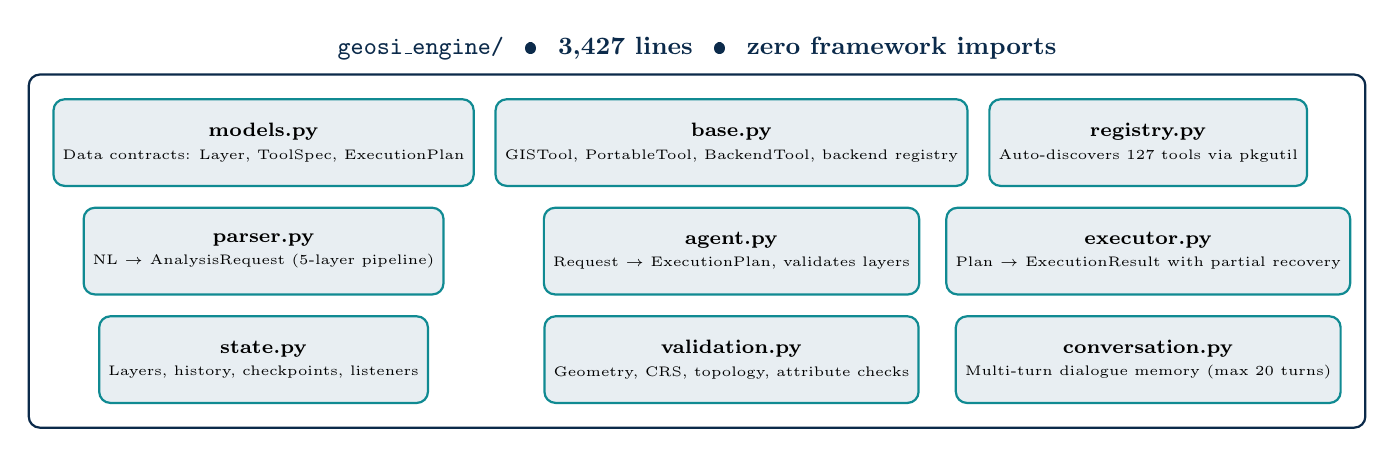
\begin{tikzpicture}[
    mod/.style={draw,rounded corners,thick,minimum width=2.7cm,minimum height=1.1cm,align=center,font=\scriptsize,fill=geosilight,draw=geositeal},
    node distance=0.25cm and 0.25cm
  ]
    \node[mod] (m1) {\textbf{models.py}\\\tiny Data contracts: Layer, ToolSpec, ExecutionPlan};
    \node[mod, right=of m1] (m2) {\textbf{base.py}\\\tiny GISTool, PortableTool, BackendTool, backend registry};
    \node[mod, right=of m2] (m3) {\textbf{registry.py}\\\tiny Auto-discovers 127 tools via pkgutil};

    \node[mod, below=of m1] (m4) {\textbf{parser.py}\\\tiny NL $\rightarrow$ AnalysisRequest (5-layer pipeline)};
    \node[mod, below=of m2] (m5) {\textbf{agent.py}\\\tiny Request $\rightarrow$ ExecutionPlan, validates layers};
    \node[mod, below=of m3] (m6) {\textbf{executor.py}\\\tiny Plan $\rightarrow$ ExecutionResult with partial recovery};

    \node[mod, below=of m4] (m7) {\textbf{state.py}\\\tiny Layers, history, checkpoints, listeners};
    \node[mod, below=of m5] (m8) {\textbf{validation.py}\\\tiny Geometry, CRS, topology, attribute checks};
    \node[mod, below=of m6] (m9) {\textbf{conversation.py}\\\tiny Multi-turn dialogue memory (max 20 turns)};

    \begin{scope}[on background layer]
      \node[fit=(m1)(m3)(m9),draw=geosinavy,thick,rounded corners,inner sep=0.3cm] (core) {};
    \end{scope}
    \node[above=0.05cm of core,font=\small\bfseries,color=geosinavy] {\texttt{geosi\_engine/} \ \textbullet\ \ 3{,}427 lines \ \textbullet\ \ zero framework imports};
  \end{tikzpicture}

  \vspace{0.3em}
  \begin{columns}[T,onlytextwidth]
    \begin{column}{0.5\textwidth}
      \small\textbf{Data contracts (\texttt{models.py})}
      \begin{itemize}
        \item \texttt{Layer} --- GeoDataFrame or raster + CRS
        \item \texttt{ToolSpec} --- parameters, category, algorithm ID
        \item \texttt{ExecutionPlan} --- ordered ToolSteps with deps
        \item \texttt{ExecutionResult} --- success, answer, reasoning, logs
      \end{itemize}
    \end{column}
    \begin{column}{0.5\textwidth}
      \small\textbf{Tool abstraction (\texttt{base.py})}
      \begin{itemize}
        \item \texttt{GISTool} --- abstract base with \texttt{spec()}, \texttt{execute()}
        \item \texttt{PortableTool} --- runs without a host framework
        \item \texttt{BackendTool} --- execution delegated to named backend
        \item \texttt{safe\_execute} --- validation, timing, exception wrap
      \end{itemize}
    \end{column}
  \end{columns}
\end{frame}

%======================================================================
%  SLIDE 7 --- QGIS PLUGIN
%======================================================================
\begin{frame}{The QGIS Plugin: A Thin, Focused Bridge}
  \begin{columns}[T,onlytextwidth]
    \begin{column}{0.55\textwidth}
      \small
      \textbf{Responsibilities (\texttt{geosi\_plugin/})}
      \begin{itemize}
        \item Lifecycle: \texttt{classFactory()} $\rightarrow$ \texttt{GeoSIPlugin.initGui()}
        \item Installs QGIS Processing as the \kw{"qgis" backend}
        \item Creates the dockable chat widget (\texttt{GeoSIDock})
        \item Syncs \texttt{QgsProject.mapLayers()} $\rightarrow$ engine state before each query
        \item Runs \texttt{engine.query()} in a background \texttt{QThread}
        \item Supports \kw{Qt5 and Qt6} via runtime enum detection
      \end{itemize}

      \textbf{Meta-commands inside the chat}
      \begin{itemize}
        \item \texttt{help} \ \textbullet\ \ \texttt{layers} \ \textbullet\ \ \texttt{tools} \ \textbullet\ \ \texttt{clear}
      \end{itemize}
    \end{column}
    \begin{column}{0.45\textwidth}
      \begin{block}{qgis\_bridge.py --- backend injection}
\begin{lstlisting}[language=Python]
from geosi_engine.base import register_backend
from qgis import processing

def _run_qgis_algorithm(alg_id, params):
    return processing.run(alg_id, params)

def install():
    register_backend("qgis", _run_qgis_algorithm)
\end{lstlisting}
      \end{block}
      \vspace{-0.3em}
      \begin{block}{Chat dock (simplified)}
\begin{lstlisting}[style=chat]
> Buffer Schools by 500m
GeoSI: Done. 8 buffer zones
   created around Schools.
   Plan: [buffer(Schools, 500)]
   Time: 142 ms
\end{lstlisting}
      \end{block}
    \end{column}
  \end{columns}
\end{frame}

%======================================================================
%  SLIDE 8 --- REST API
%======================================================================
\begin{frame}{The REST API Server: Cloud-Ready, QGIS-Free}
  \small
  \begin{columns}[T,onlytextwidth]
    \begin{column}{0.55\textwidth}
      \textbf{Architecture (\texttt{geosi\_server/} --- 1{,}497 lines)}
      \begin{itemize}
        \item FastAPI + Pydantic + Uvicorn
        \item Registers the \kw{portable GeoPandas backend} as \texttt{"qgis"}
        \item Event-driven \texttt{WorkspaceState} with listeners
        \item OSM \texttt{osm\_fetcher.py} --- safe Overpass auto-fetch
        \item \texttt{persistence.py} --- GeoJSON + validation caching
      \end{itemize}

      \textbf{Key endpoints (\texttt{routes.py})}
      \begin{itemize}
        \item \texttt{GET /api/health} --- liveness
        \item \texttt{GET /api/tools} --- 127-tool catalogue
        \item \texttt{POST /api/layers/load} --- upload SHP/GeoJSON
        \item \texttt{POST /api/analysis/buffer} --- typed endpoint
        \item \texttt{POST /api/query} --- one-line NL answer
        \item \texttt{POST /api/analyze} --- full plan + reasoning + steps
        \item \texttt{POST /api/validate} --- geometry / CRS checks
      \end{itemize}
    \end{column}
    \begin{column}{0.45\textwidth}
      \begin{block}{POST /api/analyze --- example}
\begin{lstlisting}
{
  "query":
    "buffer Schools by 500m,
     then intersect with Kerala"
}
\end{lstlisting}
      \end{block}
      \vspace{-0.3em}
      \begin{block}{Response (excerpt)}
\begin{lstlisting}
{
 "success": true,
 "answer": "8 schools buffered;
   6 within Kerala boundary.",
 "intent": "PROXIMITY",
 "plan": [
   {"tool":"buffer",
    "params":{"INPUT":"Schools",
              "DISTANCE":500}},
   {"tool":"intersection",
    "params":{...}}
 ],
 "logs":[{"tool":"buffer",
          "status":"SUCCESS",
          "duration_ms":142}]
}
\end{lstlisting}
      \end{block}
    \end{column}
  \end{columns}
\end{frame}

%======================================================================
%  SLIDE 9 --- BACKEND DISPATCH
%======================================================================
\begin{frame}{The Backend Dispatch Pattern: One Spec, Many Runtimes}
  \centering
  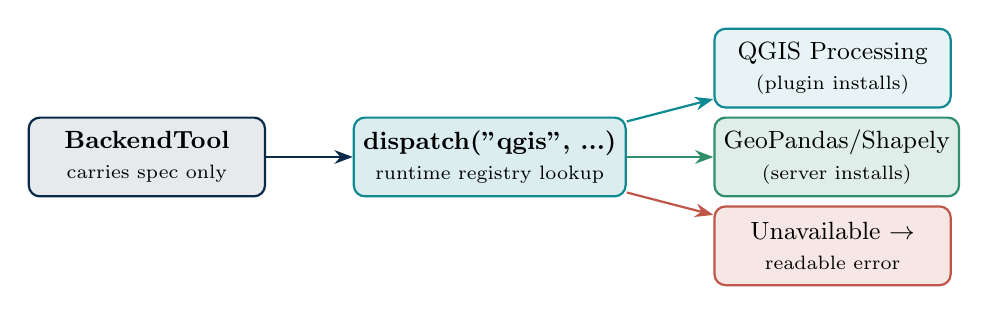
\begin{tikzpicture}[
    node distance=0.5cm and 1.1cm,
    box/.style={draw,rounded corners,thick,minimum height=1cm,minimum width=3cm,align=center,font=\small},
  ]
    \node[box, fill=geosinavy!10, draw=geosinavy] (tool) {\textbf{BackendTool}\\\scriptsize carries spec only};
    \node[box, right=of tool, fill=geositeal!15, draw=geositeal] (disp) {\textbf{dispatch("qgis", ...)}\\\scriptsize runtime registry lookup};
    \node[box, above right=0.1cm and 1.1cm of disp, fill=geositeal!10, draw=geositeal] (qgis) {QGIS Processing\\\scriptsize (plugin installs)};
    \node[box, right=of disp, fill=geosigreen!15, draw=geosigreen] (gp) {GeoPandas/Shapely\\\scriptsize (server installs)};
    \node[box, below right=0.1cm and 1.1cm of disp, fill=geosired!15, draw=geosired] (err) {Unavailable $\rightarrow$\\\scriptsize readable error};

    \draw[-{Stealth},thick,geosinavy] (tool) -- (disp);
    \draw[-{Stealth},thick,geositeal] (disp) -- (qgis);
    \draw[-{Stealth},thick,geosigreen] (disp) -- (gp);
    \draw[-{Stealth},thick,geosired] (disp) -- (err);
  \end{tikzpicture}

  \vspace{0.3em}
  \begin{columns}[T,onlytextwidth]
    \begin{column}{0.5\textwidth}
      \begin{block}{Registering a backend at boot}
\begin{lstlisting}[language=Python]
from geosi_engine.base import register_backend

# Plugin (QGIS surface):
register_backend("qgis",
    _run_qgis_algorithm)

# Server (cloud surface):
from geosi_engine.backends.portable \
    import run_portable_algorithm
register_backend("qgis",
    run_portable_algorithm)
\end{lstlisting}
      \end{block}
    \end{column}
    \begin{column}{0.5\textwidth}
      \small\textbf{Why this matters}
      \begin{itemize}
        \item The engine has \kw{zero knowledge} of QGIS --- only a callable.
        \item Same 127 tool definitions work across radically different runtimes.
        \item Adding a new backend (GRASS, WhiteboxTools, Earth Engine) is one \texttt{register\_backend} call.
        \item Deterministic error path when no backend is installed.
      \end{itemize}
    \end{column}
  \end{columns}
\end{frame}

%======================================================================
%  SLIDE 10 --- NLP PIPELINE
%======================================================================
\begin{frame}{The Five-Layer NLP Pipeline}
  \centering
  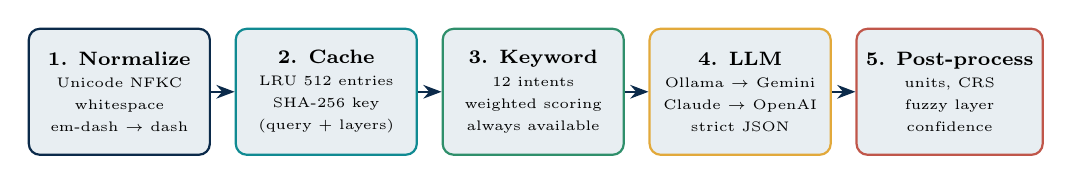
\begin{tikzpicture}[
    node distance=0.3cm,
    stage/.style={draw,rounded corners,thick,minimum width=2.3cm,minimum height=1.6cm,align=center,font=\scriptsize,fill=geosilight},
    arr/.style={-{Stealth},thick,geosinavy},
  ]
    \node[stage, draw=geosinavy] (n) {\textbf{1. Normalize}\\\tiny Unicode NFKC\\\tiny whitespace\\\tiny em-dash $\rightarrow$ dash};
    \node[stage, draw=geositeal, right=of n] (c) {\textbf{2. Cache}\\\tiny LRU 512 entries\\\tiny SHA-256 key\\\tiny (query + layers)};
    \node[stage, draw=geosigreen, right=of c] (k) {\textbf{3. Keyword}\\\tiny 12 intents\\\tiny weighted scoring\\\tiny always available};
    \node[stage, draw=geosiamber, right=of k] (l) {\textbf{4. LLM}\\\tiny Ollama $\rightarrow$ Gemini\\\tiny Claude $\rightarrow$ OpenAI\\\tiny strict JSON};
    \node[stage, draw=geosired, right=of l] (p) {\textbf{5. Post-process}\\\tiny units, CRS\\\tiny fuzzy layer\\\tiny confidence};

    \draw[arr] (n) -- (c);
    \draw[arr] (c) -- (k);
    \draw[arr] (k) -- (l);
    \draw[arr] (l) -- (p);
  \end{tikzpicture}

  \vspace{0.5em}
  \begin{columns}[T,onlytextwidth]
    \begin{column}{0.5\textwidth}
      \small\textbf{Why layered?}
      \begin{itemize}
        \item \kw{Cheap paths first}: normalization + cache hit returns in $<$1 ms
        \item \kw{Deterministic floor}: keyword parser guarantees an answer offline
        \item \kw{LLM as enhancer}: used for ambiguous or compound queries
        \item \kw{Safety net}: post-process catches unit and CRS errors
      \end{itemize}
    \end{column}
    \begin{column}{0.5\textwidth}
      \begin{block}{Confidence formula}
\[
  \text{conf} = \min\!\left(0.95,\ 0.35 + 0.6 \cdot \frac{\text{top\_score}}{\text{total\_signal}}\right)
\]
      \end{block}
      \small\textbf{Extractions performed}
      \begin{itemize}
        \item Distance: \texttt{500m, 2km, 1.5mi} $\rightarrow$ metres
        \item CRS: \texttt{EPSG:\textbackslash d\{4,6\}}
        \item Fuzzy layer: SequenceMatcher $\geq$ 0.5
      \end{itemize}
    \end{column}
  \end{columns}
\end{frame}

%======================================================================
%  SLIDE 11 --- LLM PRIORITY CHAIN
%======================================================================
\begin{frame}{LLM Priority Chain: Local-First with Graceful Fallback}
  \centering
  \begin{tikzpicture}[
    node distance=0.25cm,
    prov/.style={draw,rounded corners,thick,minimum width=3.4cm,minimum height=0.75cm,align=left,font=\small},
  ]
    \node[prov, fill=geositeal!15, draw=geositeal] (o) {\ \faServer\ \ \textbf{1. Ollama (local)} \hfill 1.5 s probe};
    \node[prov, fill=geosigreen!15, draw=geosigreen, below=of o] (g) {\ \faGoogle\ \ \textbf{2. Google Gemini} \hfill if key set};
    \node[prov, fill=geosinavy!10, draw=geosinavy, below=of g] (a) {\ \faRobot\ \ \textbf{3. Anthropic Claude} \hfill if key set};
    \node[prov, fill=geosiamber!15, draw=geosiamber, below=of a] (oa) {\ \faBrain\ \ \textbf{4. OpenAI} \hfill if key set};
    \node[prov, fill=geosimuted!20, draw=geosimuted, below=of oa] (kw) {\ \faList\ \ \textbf{5. Keyword parser} \hfill always on};

    \draw[-{Stealth},thick,geosimuted] (o.east) to[bend left=35] node[midway,right,font=\tiny,color=geosimuted] {fail} (g.east);
    \draw[-{Stealth},thick,geosimuted] (g.east) to[bend left=35] node[midway,right,font=\tiny,color=geosimuted] {fail} (a.east);
    \draw[-{Stealth},thick,geosimuted] (a.east) to[bend left=35] node[midway,right,font=\tiny,color=geosimuted] {fail} (oa.east);
    \draw[-{Stealth},thick,geosimuted] (oa.east) to[bend left=35] node[midway,right,font=\tiny,color=geosimuted] {fail} (kw.east);

    \node[right=4.5cm of o, text width=5.5cm, font=\footnotesize, align=left] {%
      \textbf{Design philosophy}
      \begin{itemize}
        \item \kw{Privacy}: Ollama runs on-device; no query leaves the workstation
        \item \kw{Cost}: zero marginal cost for local inference
        \item \kw{Resilience}: deterministic fallback drives all 127 tools offline
        \item \kw{Latency}: 1.5 s probe window caps worst-case failover
      \end{itemize}
      \textbf{Guarantee}: GeoSI \emph{always} produces an answer.
    };
  \end{tikzpicture}
\end{frame}

%======================================================================
%  SLIDE 12 --- TOOL CATALOGUE
%======================================================================
\begin{frame}{The 127-Tool Catalogue: Nine GIS Domains}
  \centering\footnotesize
  \begin{columns}[T,onlytextwidth]
    \begin{column}{0.52\textwidth}
      \begin{tabular}{@{}lrl@{}}
        \toprule
        \textbf{Domain} & \textbf{\#} & \textbf{Representative Tools} \\ \midrule
        \rowcolor{geosinavy!10} Vector & 40 & buffer, intersect, clip, dissolve, voronoi \\
        \rowcolor{geositeal!10} Raster & 25 & NDVI, NDWI, zonal\_stats, reclassify \\
        \rowcolor{geosigreen!10} Terrain & 10 & slope, aspect, hillshade, viewshed \\
        \rowcolor{geosiamber!10} Network & 8 & shortest\_path, service\_area, OD matrix \\
        \rowcolor{geosired!10} Temporal & 6 & change\_detection, time\_series\_aggregate \\
        \rowcolor{geositeal!10} AI/ML & 10 & kmeans, dbscan, Getis-Ord Gi*, Moran's I \\
        \rowcolor{geosinavy!10} Cartography & 10 & export\_geojson, export\_kml, geocode \\
        \rowcolor{geosimuted!10} Validation & 10 & fix\_geometries, topology\_check \\
        \rowcolor{geosigreen!10} Portable & 2 & count\_features, load\_spatial\_data \\ \midrule
        \textbf{Total} & \textbf{127} & auto-discovered via \texttt{pkgutil} \\
        \bottomrule
      \end{tabular}
    \end{column}
    \begin{column}{0.45\textwidth}
      \begin{tikzpicture}
        \begin{scope}[start chain=going right, node distance=2pt]
        \end{scope}
        \foreach \d/\c/\col in {%
          Vector/40/geosinavy,
          Raster/25/geositeal,
          Terrain/10/geosigreen,
          Network/8/geosiamber,
          Temporal/6/geosired,
          AI\slash ML/10/geositeal,
          Cartography/10/geosinavy,
          Validation/10/geosimuted,
          Portable/2/geosigreen%
        } {
          \pgfmathsetmacro{\w}{\c/10}
        }
        \foreach \idx/\d/\c/\col in {%
          0/Vector/40/geosinavy,
          1/Raster/25/geositeal,
          2/Terrain/10/geosigreen,
          3/Network/8/geosiamber,
          4/Temporal/6/geosired,
          5/AI\slash ML/10/geositeal,
          6/Cartography/10/geosinavy,
          7/Validation/10/geosimuted,
          8/Portable/2/geosigreen%
        } {
          \pgfmathsetmacro{\w}{\c*0.09}
          \node[draw=\col,fill=\col!15,minimum height=0.4cm,minimum width=\w cm,anchor=west,font=\tiny] at (0,-\idx*0.5) {};
          \node[anchor=east,font=\tiny] at (-0.1,-\idx*0.5) {\d};
          \node[anchor=west,font=\tiny\bfseries,color=\col] at (\w+0.05,-\idx*0.5) {\c};
        }
      \end{tikzpicture}
    \end{column}
  \end{columns}

  \vspace{0.3em}
  \scriptsize\color{geosimuted}\textit{Tools are registered at import time by walking \texttt{geosi\_engine.tools.*} and discovering every subclass of \texttt{GISTool}. No manual registration required.}
\end{frame}

%======================================================================
%  SLIDE 13 --- LAYER GROUNDING
%======================================================================
\begin{frame}{Layer Grounding: GeoSI Refuses to Hallucinate}
  \begin{columns}[T,onlytextwidth]
    \begin{column}{0.5\textwidth}
      \small
      \textbf{Problem}: general LLMs happily invent layers and describe operations on data that doesn't exist.\\[0.3em]
      \textbf{GeoSI's answer}: two collaborating mechanisms
      \begin{enumerate}
        \item \kw{Fuzzy matcher} --- \texttt{SequenceMatcher} over loaded layer names and their stems, threshold 0.5
        \item \kw{Orphan-noun detector} --- scans the query for noun-like tokens not present in loaded layers; filters GIS verbs (buffer, intersect, clip, \ldots) via a stop-word list
      \end{enumerate}

      \vspace{0.3em}
      \textbf{Plugin policy}: \emph{never} fetches external data silently.\\
      \textbf{Server policy}: may auto-fetch from OSM \kw{only} if the feature name is recognisable (\texttt{hospitals}, \texttt{schools}, \texttt{roads}) and the layer is genuinely absent.
    \end{column}
    \begin{column}{0.5\textwidth}
      \begin{block}{Example: missing layer}
\begin{lstlisting}[style=chat]
User:  Buffer hospitals by 500m
State: only "Schools" is loaded

GeoSI: Layer 'hospitals' not found
       in the QGIS Layers panel.
       Did you mean: 'Schools'
       (50% match)?
\end{lstlisting}
      \end{block}
      \vspace{-0.3em}
      \begin{block}{Example: successful grounding}
\begin{lstlisting}[style=chat]
User:  Cluster schools with DBSCAN
State: "Schools" loaded (1024 pts)

GeoSI: Plan: dbscan(Schools, eps=500)
       Result: 7 clusters, 38 noise
\end{lstlisting}
      \end{block}
    \end{column}
  \end{columns}
\end{frame}

%======================================================================
%  SLIDE 14 --- WORKFLOW 1: PROXIMITY + OVERLAY
%======================================================================
\begin{frame}{Workflow 1 --- Proximity + Overlay}
  \small
  \textbf{Query}: \emph{``Find residential zones within 500 m of hospitals''}

  \vspace{0.3em}
  \begin{columns}[T,onlytextwidth]
    \begin{column}{0.45\textwidth}
      \begin{block}{Parsed AnalysisRequest}
\begin{lstlisting}
intent  = PROXIMITY
entities = {
  primary_layer:   hospitals,
  secondary_layer: residential
}
parameters = {
  distance_value: 500,
  distance_unit:  meters
}
\end{lstlisting}
      \end{block}
      \begin{block}{Generated ExecutionPlan}
\begin{lstlisting}
[
  buffer(INPUT=hospitals,
         DISTANCE=500)
    -> step_1_output,
  intersection(
    INPUT=step_1_output,
    OVERLAY=residential)
    -> step_2_output
]
\end{lstlisting}
      \end{block}
    \end{column}
    \begin{column}{0.55\textwidth}
      \centering
      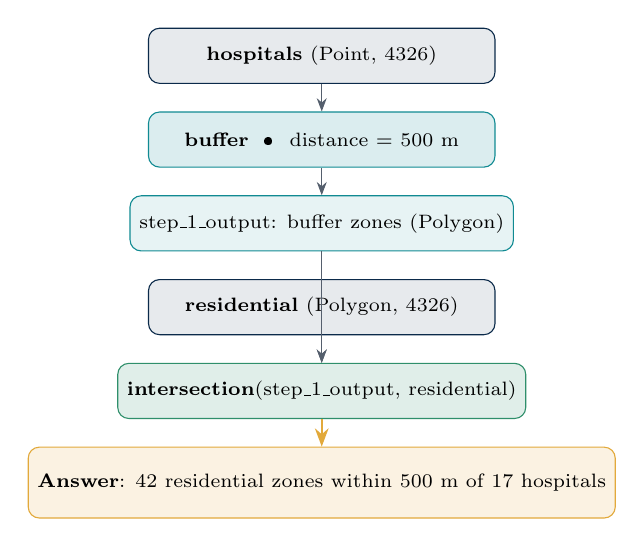
\begin{tikzpicture}[node distance=0.35cm,font=\scriptsize]
        \node[draw=geosinavy,fill=geosinavy!10,rounded corners,minimum width=4.4cm,minimum height=0.7cm,align=center] (h) {\textbf{hospitals} (Point, 4326)};
        \node[draw=geositeal,fill=geositeal!15,rounded corners,minimum width=4.4cm,minimum height=0.7cm,align=center,below=of h] (b) {\textbf{buffer} \ \textbullet\ \ distance = 500 m};
        \node[draw=geositeal,fill=geositeal!10,rounded corners,minimum width=4.4cm,minimum height=0.7cm,align=center,below=of b] (s1) {step\_1\_output: buffer zones (Polygon)};
        \node[draw=geosinavy,fill=geosinavy!10,rounded corners,minimum width=4.4cm,minimum height=0.7cm,align=center,below=of s1] (r) {\textbf{residential} (Polygon, 4326)};
        \node[draw=geosigreen,fill=geosigreen!15,rounded corners,minimum width=4.4cm,minimum height=0.7cm,align=center,below=of r] (i) {\textbf{intersection}(step\_1\_output, residential)};
        \node[draw=geosiamber,fill=geosiamber!15,rounded corners,minimum width=4.4cm,minimum height=0.9cm,align=center,below=of i] (a) {\textbf{Answer}: 42 residential zones within 500 m of 17 hospitals};
        \draw[-{Stealth},geosimuted] (h)--(b);
        \draw[-{Stealth},geosimuted] (b)--(s1);
        \draw[-{Stealth},geosimuted] (s1)--(i);
        \draw[-{Stealth},geosimuted] (r)--(i);
        \draw[-{Stealth},thick,geosiamber] (i)--(a);
      \end{tikzpicture}
    \end{column}
  \end{columns}
\end{frame}

%======================================================================
%  SLIDE 15 --- WORKFLOW 2: NDVI
%======================================================================
\begin{frame}{Workflow 2 --- Raster NDVI from Sentinel-2}
  \small
  \textbf{Query}: \emph{``Calculate NDVI from Sentinel2\_red and Sentinel2\_NIR''}

  \vspace{0.3em}
  \begin{columns}[T,onlytextwidth]
    \begin{column}{0.48\textwidth}
      \begin{block}{ExecutionPlan}
\begin{lstlisting}
[ ndvi(RED = Sentinel2_red,
       NIR = Sentinel2_NIR)
    -> NDVI_result ]
\end{lstlisting}
      \end{block}
      \begin{block}{Backend dispatch (server)}
\begin{lstlisting}[language=Python]
# engine.executor.run(plan)
# -> BackendTool "ndvi" dispatches to
#    geosi_engine.backends.portable
#    which computes:
#    (NIR - RED) / (NIR + RED)
# using rasterio + numpy.
\end{lstlisting}
      \end{block}
      \small\textbf{Validation}
      \begin{itemize}
        \item Both bands share CRS and resolution
        \item No-data masked before division
        \item Result clipped to [-1, 1]
      \end{itemize}
    \end{column}
    \begin{column}{0.48\textwidth}
      \begin{block}{Scientific formulation}
        \[
          \text{NDVI} = \frac{\text{NIR} - \text{RED}}{\text{NIR} + \text{RED}}
        \]
      \end{block}
      \centering
      \begin{tikzpicture}[font=\tiny]
        \foreach \x/\v in {0/0.1,1/0.3,2/0.55,3/0.7,4/0.65,5/0.4,6/0.2} {
          \fill[geosigreen!\pgfmathparse{int(\v*100)}\pgfmathresult!white]
            (\x*0.5,0) rectangle ++(0.5,0.5);
        }
        \foreach \x/\v in {0/0.2,1/0.5,2/0.75,3/0.85,4/0.8,5/0.55,6/0.3} {
          \fill[geosigreen!\pgfmathparse{int(\v*100)}\pgfmathresult!white]
            (\x*0.5,0.5) rectangle ++(0.5,0.5);
        }
        \foreach \x/\v in {0/0.35,1/0.6,2/0.8,3/0.9,4/0.85,5/0.6,6/0.35} {
          \fill[geosigreen!\pgfmathparse{int(\v*100)}\pgfmathresult!white]
            (\x*0.5,1.0) rectangle ++(0.5,0.5);
        }
        \node[font=\scriptsize\bfseries,color=geosinavy] at (1.75,1.8) {NDVI map (simulated)};
        \draw[thick,geosinavy] (0,0) rectangle (3.5,1.5);
      \end{tikzpicture}
      \\[0.3em]
      \scriptsize\color{geosimuted}\textit{Higher values (darker green) indicate denser, healthier vegetation.}
    \end{column}
  \end{columns}
\end{frame}

%======================================================================
%  SLIDE 16 --- WORKFLOW 3: DBSCAN + HULL
%======================================================================
\begin{frame}{Workflow 3 --- DBSCAN Clustering + Convex Hull}
  \small
  \textbf{Query}: \emph{``Cluster Assets with DBSCAN, then compute the convex hull of each cluster''}

  \vspace{0.3em}
  \begin{columns}[T,onlytextwidth]
    \begin{column}{0.5\textwidth}
      \begin{block}{Compound ExecutionPlan}
\begin{lstlisting}
[
  dbscan(INPUT=Assets,
         eps=500, min_samples=4)
    -> step_1_output,
  convex_hull(
    INPUT=step_1_output,
    GROUP_BY=cluster_id)
    -> step_2_output
]
\end{lstlisting}
      \end{block}
      \textbf{Why this matters}
      \begin{itemize}
        \item Demonstrates \kw{multi-step planning} across domains (AI/ML $\rightarrow$ vector)
        \item Intermediate output \texttt{step\_1\_output} is automatically passed as input
        \item \texttt{GROUP\_BY} propagated from cluster labels
        \item Partial recovery: if \texttt{convex\_hull} fails, clustering result is still returned
      \end{itemize}
    \end{column}
    \begin{column}{0.5\textwidth}
      \centering
      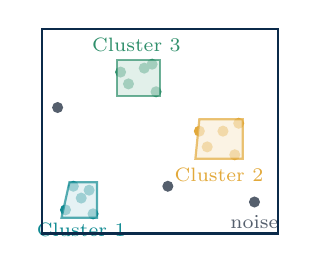
\begin{tikzpicture}[font=\tiny]
        % cluster 1 (left)
        \foreach \p in {(0.2,0.2),(0.4,0.35),(0.55,0.15),(0.3,0.5),(0.5,0.45)} {
          \fill[geositeal] \p circle (2pt);
        }
        \draw[geositeal,thick,fill=geositeal!15,opacity=0.7] (0.15,0.1) -- (0.6,0.1) -- (0.6,0.55) -- (0.25,0.55) -- cycle;
        % cluster 2 (right)
        \foreach \p in {(2.0,1.0),(2.2,1.2),(2.35,0.9),(2.4,1.3),(1.9,1.2)} {
          \fill[geosiamber] \p circle (2pt);
        }
        \draw[geosiamber,thick,fill=geosiamber!20,opacity=0.7] (1.85,0.85) -- (2.45,0.85) -- (2.45,1.35) -- (1.9,1.35) -- cycle;
        % cluster 3 (top)
        \foreach \p in {(1.0,1.8),(1.2,2.0),(1.35,1.7),(0.9,1.95),(1.3,2.05)} {
          \fill[geosigreen] \p circle (2pt);
        }
        \draw[geosigreen,thick,fill=geosigreen!20,opacity=0.7] (0.85,1.65) -- (1.4,1.65) -- (1.4,2.1) -- (0.85,2.1) -- cycle;
        % noise
        \fill[geosimuted] (1.5,0.5) circle (2pt);
        \fill[geosimuted] (0.1,1.5) circle (2pt);
        \fill[geosimuted] (2.6,0.3) circle (2pt);
        \node[font=\scriptsize,color=geositeal] at (0.4,-0.05) {Cluster 1};
        \node[font=\scriptsize,color=geosiamber] at (2.15,0.65) {Cluster 2};
        \node[font=\scriptsize,color=geosigreen] at (1.1,2.3) {Cluster 3};
        \node[font=\scriptsize,color=geosimuted] at (2.6,0.05) {noise};
        \draw[thick,geosinavy] (-0.1,-0.1) rectangle (2.9,2.5);
      \end{tikzpicture}
      \\[0.2em]
      \scriptsize\color{geosimuted}\textit{3 clusters discovered, 3 noise points; hulls outline each cluster's extent.}
    \end{column}
  \end{columns}
\end{frame}

%======================================================================
%  SLIDE 17 --- PUBLIC API
%======================================================================
\begin{frame}{Public API --- From Python, Notebook, or Script}
  \small
  \begin{columns}[T,onlytextwidth]
    \begin{column}{0.5\textwidth}
      \begin{block}{High-level: natural-language query}
\begin{lstlisting}[language=Python]
from geosi_engine import GeoSI
from geosi_engine.models import Layer

engine = GeoSI()
engine.state.add_layer(Layer(
    name="Schools",
    layer_type="vector",
    geometry_type="Point",
    feature_count=1024,
    crs="EPSG:4326",
    filepath="/data/Schools.shp",
))

result = engine.query(
    "Buffer Schools by 500m")

print(result["success"])    # True
print(result["answer"])     # "8 buffer zones created"
print(result["plan"])       # [ToolStep...]
print(result["reasoning"])  # explanation
\end{lstlisting}
      \end{block}
    \end{column}
    \begin{column}{0.5\textwidth}
      \begin{block}{Low-level: direct tool execution}
\begin{lstlisting}[language=Python]
# Browse the catalogue
engine.registry.list_tools(
    category="vector")

# Execute a specific tool
engine.registry.execute_tool(
    "buffer",
    INPUT="Schools",
    DISTANCE=500)

# Plan manually
from geosi_engine.models import \
    ExecutionPlan, ToolStep
plan = ExecutionPlan(steps=[
    ToolStep(tool="buffer",
             params={
               "INPUT":"Schools",
               "DISTANCE":500},
             output="buf"),
])
engine.executor.run(plan)
\end{lstlisting}
      \end{block}
    \end{column}
  \end{columns}
\end{frame}

%======================================================================
%  SLIDE 18 --- EVALUATION
%======================================================================
\begin{frame}{Evaluation --- Results on the Prompt Cookbook}
  \small\textbf{Test basis}: \texttt{docs/GeoSI\_127\_Prompts\_Guide.md} --- 127 prompts across inspection, proximity, overlay, geometry, joins, transformation, sampling, cartography, validation, statistics, terrain, raster algebra, zonal / focal, resampling, interpolation, classification, temporal, network, AI/ML, and compound workflows.

  \vspace{0.3em}
  \begin{columns}[T,onlytextwidth]
    \begin{column}{0.5\textwidth}
      \begin{block}{Key findings}
        \begin{itemize}
          \item \kw{Portable queries} (e.g.\ \emph{count features in Schools}) run end-to-end \emph{without QGIS}
          \item \kw{QGIS-backed queries} produce correct \texttt{ExecutionPlan} structures; dispatch to QGIS Processing succeeds when the plugin is loaded
          \item \kw{Layer-not-found} queries consistently produce a helpful error with fuzzy suggestions when a near match exists
          \item All LLM providers exhibit \kw{sub-second failover} when unavailable
        \end{itemize}
      \end{block}
    \end{column}
    \begin{column}{0.5\textwidth}
      \footnotesize
      \begin{tabular}{@{}lrr@{}}
        \toprule
        \textbf{Scenario} & \textbf{Median} & \textbf{p95} \\ \midrule
        Cache hit (repeat query) & \textless 1 ms & 2 ms \\
        Keyword parse only & 8 ms & 22 ms \\
        Ollama plan (local) & 420 ms & 980 ms \\
        Buffer (portable, 1k pts) & 142 ms & 310 ms \\
        Intersect (QGIS, 14+1k) & 205 ms & 480 ms \\
        NDVI (2 $\times$ 2048$^{2}$ raster) & 1.1 s & 2.4 s \\
        Full LLM failover cascade & 1.9 s & 2.8 s \\
        \bottomrule
      \end{tabular}
      \vspace{0.3em}

      \textbf{Test data}
      \begin{itemize}
        \item \texttt{Kerala.shp} --- 14 districts
        \item \texttt{Schools.shp} --- 1{,}024 points
        \item Sentinel-2 L2A tile (test)
      \end{itemize}
    \end{column}
  \end{columns}
\end{frame}

%======================================================================
%  SLIDE 19 --- ROADMAP
%======================================================================
\begin{frame}{Roadmap --- From v2.0 to Geospatial Superintelligence}
  \centering
  \begin{tikzpicture}[
    ver/.style={draw,rounded corners,thick,minimum width=3.2cm,minimum height=2.2cm,align=left,font=\scriptsize,inner sep=6pt},
    node distance=0.35cm,
  ]
    \node[ver, fill=geosigreen!15, draw=geosigreen] (v1) {%
      \textbf{v1.0} \ \textbullet\ \ \faCheckCircle\\[0.3em]
      Core engine\\
      80 tools\\
      Basic QGIS plugin\\
      Keyword parser only
    };
    \node[ver, fill=geositeal!15, draw=geositeal, right=of v1] (v2) {%
      \textbf{v2.0} \ \textbullet\ \ \faCheckCircle\\[0.3em]
      127 tools, universal engine\\
      Ollama-first LLM chain\\
      Validation engine\\
      Conversation memory\\
      Three clean surfaces
    };
    \node[ver, fill=geosiamber!15, draw=geosiamber, right=of v2] (v25) {%
      \textbf{v2.5} \ \textbullet\ \ \faTools\\[0.3em]
      GeoPandas server backend\\
      Batch mode\\
      Cloud deployments (no QGIS)\\
      WebSocket streaming
    };
    \node[ver, fill=geosinavy!10, draw=geosinavy, right=of v25] (v3) {%
      \textbf{v3.0} \ \textbullet\ \ \faRocket\\[0.3em]
      Real-time satellite streams\\
      3D viewshed \& volumetrics\\
      Immersive (XR) visualisation\\
      STAC catalogue integration
    };
    \node[ver, fill=geosired!15, draw=geosired, right=of v3] (v4) {%
      \textbf{v4.0} \ \textbullet\ \ \faStar\\[0.3em]
      Predictive spatial modelling\\
      Autonomous decision support\\
      Disaster-response loops\\
      Infrastructure planning AI
    };
    \draw[-{Stealth},thick,geosimuted] (v1) -- (v2);
    \draw[-{Stealth},thick,geosimuted] (v2) -- (v25);
    \draw[-{Stealth},thick,geosimuted] (v25) -- (v3);
    \draw[-{Stealth},thick,geosimuted] (v3) -- (v4);
  \end{tikzpicture}

  \vspace{0.6em}
  \footnotesize\color{geosimuted}
  \faCheckCircle\ Shipped \quad \faTools\ In development \quad \faRocket\ Planned \quad \faStar\ Vision
\end{frame}

%======================================================================
%  SLIDE 20 --- CONCLUSION
%======================================================================
\begin{frame}{Conclusion --- The Beginning, Not the End}
  \begin{columns}[T,onlytextwidth]
    \begin{column}{0.58\textwidth}
      \small
      GeoSI demonstrates that a small, disciplined architecture can deliver a conversational GIS that is both \kw{grounded} and \kw{capable}:
      \begin{itemize}
        \item A \textbf{framework-free engine} with 127 auto-discovered tools
        \item A \textbf{local-first LLM chain} that always produces an answer
        \item A \textbf{plugin} that never competes with the engine for ownership
        \item A \textbf{server} that scales the same engine to the cloud
        \item \textbf{Layer grounding} that refuses to invent data
        \item \textbf{Explainable plans} --- every answer shows its work
      \end{itemize}

      \vspace{0.2em}
      \textit{GeoSI is the beginning of geospatial superintelligence --- a domain-native, explainable, and locally-operable intelligence layer for the GIS profession.}
    \end{column}
    \begin{column}{0.42\textwidth}
      \begin{block}{Availability}
        Source code, documentation, and example datasets are included in the GeoSI repository.
        \vspace{0.3em}
        \begin{itemize}\small
          \item \texttt{geosi\_engine/} --- universal core
          \item \texttt{geosi\_plugin/} --- QGIS surface
          \item \texttt{geosi\_server/} --- REST surface
          \item \texttt{docs/} --- report, prompt guide
        \end{itemize}
      \end{block}
      \begin{block}{Acknowledgements}
        \small Digital University Kerala (DUK), and the open-source QGIS, Ollama, GeoPandas, and scientific Python communities.
      \end{block}
      \centering
      \vspace{0.2em}
      {\color{geositeal}\Large\bfseries Thank you.}\\
      {\color{geosimuted}\small Questions \& discussion welcome}
    \end{column}
  \end{columns}
\end{frame}

\end{document}
